\section{Introduction}\label{sec:intro}

\begin{figure}[t]
    \begin{subfigure}[b]{0.23\textwidth}
    \centering
    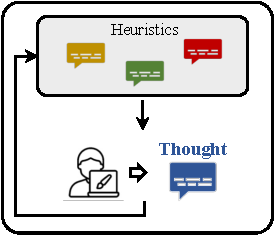
\includegraphics[width=0.9\textwidth]{figures/teaser1.pdf}
    \caption{Manual Design}
    \end{subfigure} \hfill
    \begin{subfigure}[b]{0.23\textwidth}
    \centering
    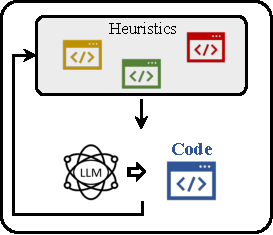
\includegraphics[width=0.9\textwidth]{figures/teaser_funsearch.pdf}
    \caption{Evol. of codes (FunSearch)}
    \end{subfigure}\hfill
    \centering
    \begin{subfigure}[b]{0.48\textwidth}
    \centering
    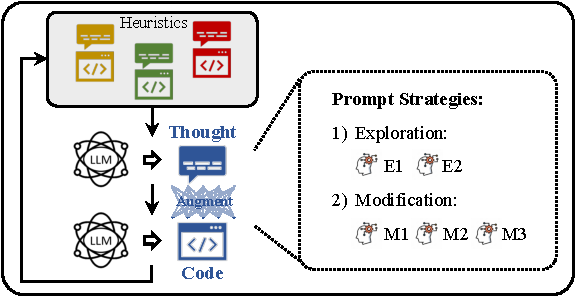
\includegraphics[width=0.9\textwidth]{figures/teasear_ours.pdf}
    \caption{Evolution of both thoughts and codes (EoH, ours)}
    \end{subfigure}
    \caption{Heuristic design often (a) relies on human expertise with reasoning over thoughts; recent progress has been made on (b) search over the space of codes; while (c) our method evolves both \textit{thoughts} and \textit{codes} using large language models.\label{fig:enter-label}} 
\end{figure}


Heuristics are commonly used for tackling complex search and optimization problems. 
%
Over the last several decades, much effort has been devoted to designing effective heuristics, leading to simulated annealing~\cite{van1987simulated}, tabu search~\cite{glover1998tabu}, and iterated local search~\cite{lourencco2003iterated}, among many other methods~\cite{mart2018handbook}. 
% 
These hand-crafted methods have been successfully used in a wide spectrum of real-world applications. However, different applications may require different algorithms and/or algorithm configurations. Manually designing, modifying, and configuring a heuristic for a given problem can be very labor-intensive and demands rich expert experience. This is a bottleneck in many application domains. To address this issue, Automatic Heuristic Design (AHD) has been proposed and become an active research area~\cite{burke2013hyper,stutzle2019automated}. 
%It is often not only very labor-intensive but also requires some good intuition and rich expert experience to manually design, modify and/or configure a heuristic for a given problem.
%
AHD selects, tunes, or constructs effective heuristics for a given problem class automatically.  
%
Genetic Programming (GP) has been used in AHD~\cite{langdon2013foundations,zhang2023survey}. GP requires a set of permissible primitives or mutation operations for defining and generating heuristics. It could be very difficult to construct a suitable set in practice~\cite{o2010open}.

% \iffalse
% Genetic programming has been used to evolve new heuristics automatically~\cite{langdon2013foundations}. Their resultant algorithms are often explainable and perform well in various domains~\cite{mei2022explainable,zhang2023survey}.  However, a major issue is that algorithmic components still require manual crafting with domain knowledge. \fi

It is believed that Large Language Models (LLMs) ~\cite{chen2021evaluating, austin2021program, li2023starcoder} could be a powerful tool for generating new ideas and heuristics. 
%
% LLMs have received significant attention due to their zero/few-shot ability to perform diverse tasks~\cite{zhao2023survey,kasneci2023chatgpt,zhang2023automl,zhao2023large}. FF
%
However, standalone LLMs with prompt engineering can be insufficient for producing novel and useful ideas beyond existing knowledge~\cite{mahowald2023dissociating}.
%
Some attempts have been made to couple LLMs with Evolutionary Computation (EC) methods to produce heuristics in an automatic manner~\cite{yang2023large, meyerson2023language, chen2023evoprompting}. 
%
One representative work is FunSearch~\cite{romera2024mathematical}. 
%
It models AHD as a search problem in the space of functions, where each function is a heuristic represented by a program and it uses LLMs in an evolutionary framework to iteratively improve the quality of generated functions. FunSearch has been applied on several problems with great success. However, its mechanism is not very efficient and it needs a very large amount of computational resources to generate a quality heuristic. 


In this paper, we present a new evolutionary paradigm, dubbed \emph{Evolution of Heuristic (\ourmethod{})}~\footnote{Our work and its preliminary version~\cite{liu2023algorithm} were developed independently of \citet{romera2024mathematical}.}, to take advantage of both LLMs and EC for AHD.
%~\footnote{Our work was developed independently of \cite{romera2024mathematical}.  Actually, the first version of our work \cite{liu2023algorithm} was published online two weeks before it.}
%
Specifically, we leverage a linguistic description, referred to as a \emph{thought}, to represent a high-level idea (i.e., key logic) of a heuristic. 
%
Then, a corresponding \emph{code} representation, i.e., an executable implementation of a heuristic, is generated via an LLM.
%
We propose an evolutionary framework to simultaneously evolve the thoughts and codes of heuristics in a cooperative manner.
%
We demonstrate that the LLM-assisted evolution of both thoughts and codes with curated prompts leads to state-of-the-art AHD performance.
%
We expect that \ourmethod{} serves as a step towards efficient and automatic algorithm design. 

%
In summary, our contributions are as follows:
\begin{itemize}
%[leftmargin=1em,parsep=0pt,topsep=0pt]
    \item We propose \ourmethod{}, a novel paradigm that uses LLMs to evolution both thoughts and codes for the automatic design of heuristics with minimum hand-craft design and no domain model training.
    %without domain knowledge about the problem at hand or its plausible solution.
    %
    \item We develop several simple yet effective prompt strategies to guide LLMs toward generating more diverse and effective heuristics. These prompt strategies are generally applicable to other LLM-assisted search methods.  
    %
    \item We comprehensively evaluate \ourmethod{} on three widely-studied combinatorial optimization benchmark problems.  We demonstrate that \ourmethod{} outperforms many existing AHD methods. In particular, \ourmethod{} identifies heuristics with better performance than those designed by FunSearch. \ourmethod{} uses much fewer queries to LLMs than FunSearch on online bin packing problem.

\end{itemize}
\vspace{1pt}


